\chapter{项目要点}

    \section{项目目标}

        本项目的目标是实现\textbf{吉他扫弦}功能,吉他扫弦可以概括为\textbf{左手和弦,右手扫弦}。

        扫弦是吉他的\textbf{特色}之一,容易上手,结合声乐可以\textbf{弹唱}大部分流行歌曲,对\textbf{精度}要求不太高,同时结合指弹,可以给用户带来完整的用户体验。
        
    \section{右手扫弦}

        在吉他弹奏过程中,右手按照音乐的节拍扫动没有被禁用的弦,在左手的和弦下,便会发出一段精美的乐音。

        \image[6in]{e}{右手扫弦}

        六根弦位置固定

        利用右手的位置、走向、高度等信息

        连续同方向扫弦问题

        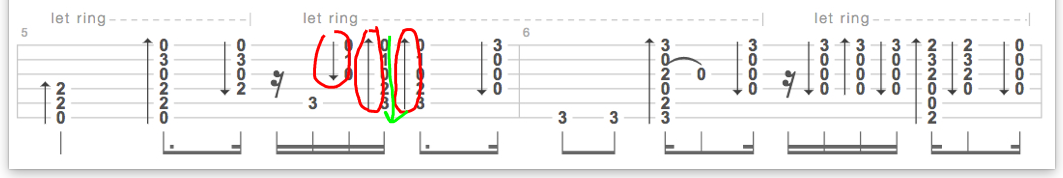
\includegraphics[width=\textwidth]{strumming}

    \section{左手和弦}

        为了能扫出不同和弦,我们需要左手来选择和弦。在普通吉他中,左手用手指在按下六根弦中的\
        不同离散的位置(称为“品”),也可以不按。这样不同的按法,就能让右手扫弦时产生不同的和弦声音。

        \image[6in]{f}{左手和弦}

        为了解决左手和弦问题,我们提出了以下几个算法。

        \subsection{九宫格算法}

        将和弦抽象成一个个按钮,均匀的分布在空间的9个点上,利用左手食指点击动作选择和弦以代替整个手的和弦动作。

        优点是操作方便,容易上手,实现简单。缺点是可用和弦数量有限。

        \subsection{1-近邻算法}

        左手每个手指分别获取位置后,判断每个手指是否按到弦。

        优点是实现简单,适合指弹。缺点是无法利用和弦固定位置的信息。

        \subsection{条件概率算法}

        参考《ATK: Enabling Ten-Finger Freehand Typing in Air Based on 3D Hand Tracking Data》论文,主要是采用条件期望公式,利用某个和弦下,输入的先验概率分布。

        $$P(C|I)=\frac{P(C) \times P(I|C)}{P(I)}\propto P(C)\times P(I|C)$$

        公式中I为input(输入),C为chord(和弦)。

        优点是能充分利用和弦信息,把每个和弦看做word,能大大提高准确率。缺点是实现较复杂,需要事先得到$P(I|C)$。

        \subsection{神经网络算法}

        收集左手数据,利用左手数据的信息训练出一个神经网络(MLP),通过训练好的神经网络进行分类。

        优点是学科交叉,神经网络算法准确率一般较高。缺点是需要收集大量数据,且容易过拟合开发者的弹奏习惯。

        \subsection{附加算法}

        \begin{enumerate}
            \item{加入手指信息}:一个和弦中按的弦与手指对应,可以加入输入端点位置对应的手指信息提高准确率。
            \item{预测和弦进行}:一般乐曲和弦的进行都是有规律的,如C-G-Am-Em-F-G-C,可以加入乐曲进行信息提高准确率。
            \item{加入反馈信息}:软件方面视觉上给出合适的反馈,从而使用户可以在弹奏中学习适应。
        \end{enumerate}

        \subsection{最终算法}

        由于左手和弦手掌朝向身体内侧,在桌面上放置Leap Motion时无法捕捉到左手手指的信息,并且由于空间中没有标\
        “品”的位置,非常容易弹错。因此为了容易上手,我们使用大多数吉他应用app的套路,\
        就是用预设和弦组合,然后以button的形式让用户选择。

        我们选择C调的常用和弦以九宫格的形式呈现给用户,对应到空间中就是一个虚拟的九宫格\
        ,左手用点击来选择和弦。我们用了选择确认反馈提升用户体验。
